% Options for packages loaded elsewhere
\PassOptionsToPackage{unicode}{hyperref}
\PassOptionsToPackage{hyphens}{url}
%
\documentclass[
]{book}
\usepackage{amsmath,amssymb}
\usepackage{lmodern}
\usepackage{iftex}
\ifPDFTeX
  \usepackage[T1]{fontenc}
  \usepackage[utf8]{inputenc}
  \usepackage{textcomp} % provide euro and other symbols
\else % if luatex or xetex
  \usepackage{unicode-math}
  \defaultfontfeatures{Scale=MatchLowercase}
  \defaultfontfeatures[\rmfamily]{Ligatures=TeX,Scale=1}
\fi
% Use upquote if available, for straight quotes in verbatim environments
\IfFileExists{upquote.sty}{\usepackage{upquote}}{}
\IfFileExists{microtype.sty}{% use microtype if available
  \usepackage[]{microtype}
  \UseMicrotypeSet[protrusion]{basicmath} % disable protrusion for tt fonts
}{}
\makeatletter
\@ifundefined{KOMAClassName}{% if non-KOMA class
  \IfFileExists{parskip.sty}{%
    \usepackage{parskip}
  }{% else
    \setlength{\parindent}{0pt}
    \setlength{\parskip}{6pt plus 2pt minus 1pt}}
}{% if KOMA class
  \KOMAoptions{parskip=half}}
\makeatother
\usepackage{xcolor}
\usepackage{color}
\usepackage{fancyvrb}
\newcommand{\VerbBar}{|}
\newcommand{\VERB}{\Verb[commandchars=\\\{\}]}
\DefineVerbatimEnvironment{Highlighting}{Verbatim}{commandchars=\\\{\}}
% Add ',fontsize=\small' for more characters per line
\usepackage{framed}
\definecolor{shadecolor}{RGB}{248,248,248}
\newenvironment{Shaded}{\begin{snugshade}}{\end{snugshade}}
\newcommand{\AlertTok}[1]{\textcolor[rgb]{0.94,0.16,0.16}{#1}}
\newcommand{\AnnotationTok}[1]{\textcolor[rgb]{0.56,0.35,0.01}{\textbf{\textit{#1}}}}
\newcommand{\AttributeTok}[1]{\textcolor[rgb]{0.77,0.63,0.00}{#1}}
\newcommand{\BaseNTok}[1]{\textcolor[rgb]{0.00,0.00,0.81}{#1}}
\newcommand{\BuiltInTok}[1]{#1}
\newcommand{\CharTok}[1]{\textcolor[rgb]{0.31,0.60,0.02}{#1}}
\newcommand{\CommentTok}[1]{\textcolor[rgb]{0.56,0.35,0.01}{\textit{#1}}}
\newcommand{\CommentVarTok}[1]{\textcolor[rgb]{0.56,0.35,0.01}{\textbf{\textit{#1}}}}
\newcommand{\ConstantTok}[1]{\textcolor[rgb]{0.00,0.00,0.00}{#1}}
\newcommand{\ControlFlowTok}[1]{\textcolor[rgb]{0.13,0.29,0.53}{\textbf{#1}}}
\newcommand{\DataTypeTok}[1]{\textcolor[rgb]{0.13,0.29,0.53}{#1}}
\newcommand{\DecValTok}[1]{\textcolor[rgb]{0.00,0.00,0.81}{#1}}
\newcommand{\DocumentationTok}[1]{\textcolor[rgb]{0.56,0.35,0.01}{\textbf{\textit{#1}}}}
\newcommand{\ErrorTok}[1]{\textcolor[rgb]{0.64,0.00,0.00}{\textbf{#1}}}
\newcommand{\ExtensionTok}[1]{#1}
\newcommand{\FloatTok}[1]{\textcolor[rgb]{0.00,0.00,0.81}{#1}}
\newcommand{\FunctionTok}[1]{\textcolor[rgb]{0.00,0.00,0.00}{#1}}
\newcommand{\ImportTok}[1]{#1}
\newcommand{\InformationTok}[1]{\textcolor[rgb]{0.56,0.35,0.01}{\textbf{\textit{#1}}}}
\newcommand{\KeywordTok}[1]{\textcolor[rgb]{0.13,0.29,0.53}{\textbf{#1}}}
\newcommand{\NormalTok}[1]{#1}
\newcommand{\OperatorTok}[1]{\textcolor[rgb]{0.81,0.36,0.00}{\textbf{#1}}}
\newcommand{\OtherTok}[1]{\textcolor[rgb]{0.56,0.35,0.01}{#1}}
\newcommand{\PreprocessorTok}[1]{\textcolor[rgb]{0.56,0.35,0.01}{\textit{#1}}}
\newcommand{\RegionMarkerTok}[1]{#1}
\newcommand{\SpecialCharTok}[1]{\textcolor[rgb]{0.00,0.00,0.00}{#1}}
\newcommand{\SpecialStringTok}[1]{\textcolor[rgb]{0.31,0.60,0.02}{#1}}
\newcommand{\StringTok}[1]{\textcolor[rgb]{0.31,0.60,0.02}{#1}}
\newcommand{\VariableTok}[1]{\textcolor[rgb]{0.00,0.00,0.00}{#1}}
\newcommand{\VerbatimStringTok}[1]{\textcolor[rgb]{0.31,0.60,0.02}{#1}}
\newcommand{\WarningTok}[1]{\textcolor[rgb]{0.56,0.35,0.01}{\textbf{\textit{#1}}}}
\usepackage{longtable,booktabs,array}
\usepackage{calc} % for calculating minipage widths
% Correct order of tables after \paragraph or \subparagraph
\usepackage{etoolbox}
\makeatletter
\patchcmd\longtable{\par}{\if@noskipsec\mbox{}\fi\par}{}{}
\makeatother
% Allow footnotes in longtable head/foot
\IfFileExists{footnotehyper.sty}{\usepackage{footnotehyper}}{\usepackage{footnote}}
\makesavenoteenv{longtable}
\usepackage{graphicx}
\makeatletter
\def\maxwidth{\ifdim\Gin@nat@width>\linewidth\linewidth\else\Gin@nat@width\fi}
\def\maxheight{\ifdim\Gin@nat@height>\textheight\textheight\else\Gin@nat@height\fi}
\makeatother
% Scale images if necessary, so that they will not overflow the page
% margins by default, and it is still possible to overwrite the defaults
% using explicit options in \includegraphics[width, height, ...]{}
\setkeys{Gin}{width=\maxwidth,height=\maxheight,keepaspectratio}
% Set default figure placement to htbp
\makeatletter
\def\fps@figure{htbp}
\makeatother
\setlength{\emergencystretch}{3em} % prevent overfull lines
\providecommand{\tightlist}{%
  \setlength{\itemsep}{0pt}\setlength{\parskip}{0pt}}
\setcounter{secnumdepth}{5}
\usepackage{booktabs}
\usepackage{amsthm}
\makeatletter
\def\thm@space@setup{%
  \thm@preskip=8pt plus 2pt minus 4pt
  \thm@postskip=\thm@preskip
}
\makeatother
\usepackage{booktabs}
\usepackage{longtable}
\usepackage{array}
\usepackage{multirow}
\usepackage{wrapfig}
\usepackage{float}
\usepackage{colortbl}
\usepackage{pdflscape}
\usepackage{tabu}
\usepackage{threeparttable}
\usepackage{threeparttablex}
\usepackage[normalem]{ulem}
\usepackage{makecell}
\usepackage{xcolor}
\ifLuaTeX
  \usepackage{selnolig}  % disable illegal ligatures
\fi
\usepackage[]{natbib}
\bibliographystyle{apalike}
\IfFileExists{bookmark.sty}{\usepackage{bookmark}}{\usepackage{hyperref}}
\IfFileExists{xurl.sty}{\usepackage{xurl}}{} % add URL line breaks if available
\urlstyle{same} % disable monospaced font for URLs
\hypersetup{
  pdftitle={Center for Conservation Biology \textbar{} UC Riverside},
  pdfauthor={Lynn Sweet \textbar{} Principal Investigator, Assistant Research Ecologist; Julia Parish \textbar{} Data Science Intern},
  hidelinks,
  pdfcreator={LaTeX via pandoc}}

\title{Center for Conservation Biology \textbar{} UC Riverside}
\usepackage{etoolbox}
\makeatletter
\providecommand{\subtitle}[1]{% add subtitle to \maketitle
  \apptocmd{\@title}{\par {\large #1 \par}}{}{}
}
\makeatother
\subtitle{Installation Guide}
\author{Lynn Sweet \textbar{} Principal Investigator, Assistant Research Ecologist \and Julia Parish \textbar{} Data Science Intern}
\date{2022-07-22}

\begin{document}
\maketitle

{
\setcounter{tocdepth}{1}
\tableofcontents
}
\hypertarget{informational-resource-for-ccb-faculty-staff}{%
\chapter*{Informational Resource for CCB Faculty \& Staff}\label{informational-resource-for-ccb-faculty-staff}}
\addcontentsline{toc}{chapter}{Informational Resource for CCB Faculty \& Staff}

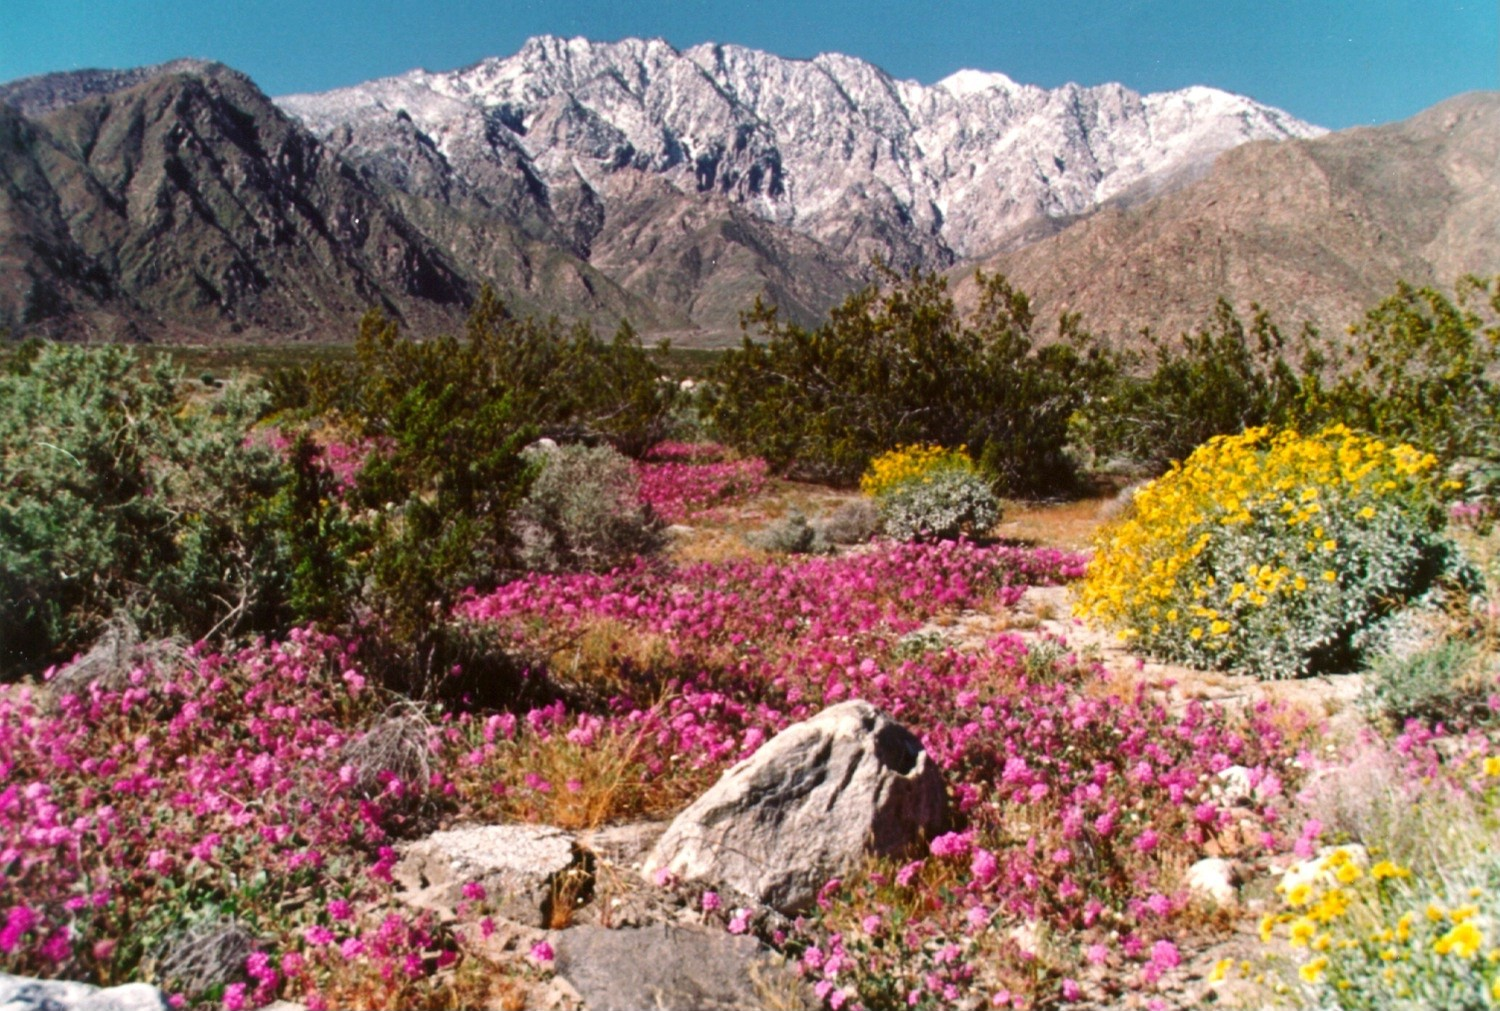
\includegraphics[width=20.83in]{images/cvmc_billhavert}

Chino Canyon Wildflowers, Coachella Valley, California.
\textbf{Image Credit:} Coachella Valley Mountains Conservancy: \emph{Bill Havert}

\begin{center}
\includegraphics[width=12.85in]{images/ucrccb} \end{center}

\hypertarget{intro}{%
\chapter{Introduction}\label{intro}}

This is an installation and account set up reference guide for the Center for Conservation Biology team. Team members may contribute to this reference file as we expand the tools utlizied during research efforts.

\hypertarget{computer-requirements}{%
\section{Computer requirements}\label{computer-requirements}}

Work computers (laptop or desktop) operating systems should either be Windows or macOS. Please note that Windows based machine it required to run ESRI ArcDesktop and ArcPro software. Both Windows and macOS may utilize ESRI ArcOnline tools.

For \textbf{Mac} users, update macOS to the newest supported version. Navigate to System Preferences --\textgreater{} Software Update.

For \textbf{PC} users, ensure you have Windows 10 or 11 installed. If not, request a Windows key from UCR IT at \href{https://ucrsupport.service-now.com/ucr_portal?id=ucr_home}{UC Riverside ServiceLink}

\hypertarget{software}{%
\section{Software}\label{software}}

Software covered in this reference guide includes:

\begin{itemize}
\tightlist
\item
  git
\item
  GitHub
\item
  Google Apps
\item
  R
\item
  RStudio

  \begin{itemize}
  \tightlist
  \item
    Quarto
  \item
    Bookdown
  \end{itemize}
\item
  Slack
\item
  Trello

  \begin{itemize}
  \tightlist
  \item
    Trello 4 Slack
  \end{itemize}
\item
  Zotero
\end{itemize}

\begin{center}\rule{0.5\linewidth}{0.5pt}\end{center}

Thank you to UC Santa Barbara's Bren School of Environmental Science \& Management and National Center for Ecological Analysis and Synthesis (NCEAS) staff for providing many of the resources listed in this reference guide. Information was made available on the \href{https://github.com/UCSB-MEDS}{UCSB-MEDS GitHub page}.

\hypertarget{bookdown}{%
\chapter{Bookdown Guide}\label{bookdown}}

The first step to edit and add to this bookdown is to install the \textbf{bookdown} package from CRAN or Github:

\begin{Shaded}
\begin{Highlighting}[]
\FunctionTok{install.packages}\NormalTok{(}\StringTok{"bookdown"}\NormalTok{)}
\CommentTok{\# or the development version}
\CommentTok{\# devtools::install\_github(\textquotesingle{}rstudio/bookdown\textquotesingle{})}
\end{Highlighting}
\end{Shaded}

\hypertarget{primary-reference-resources}{%
\section{Primary Reference Resources}\label{primary-reference-resources}}

Here is a list of resources to learn how to use and edit in bookdown

\begin{itemize}
\tightlist
\item
  \href{https://bookdown.org/}{Bookdown Package Documentation}
\item
  \href{https://bookdown.org/yihui/bookdown/}{Authoring Books with R Markdown}
\item
  \href{https://bookdown.org/yihui/rmarkdown-cookbook/}{R Markdown Cookbook}
\item
  \href{https://bookdown.org/yihui/rmarkdown/}{R Markdown: The Definitive Guide}
\end{itemize}

\begin{center}\rule{0.5\linewidth}{0.5pt}\end{center}

\textbf{The following information is directly taken from the \emph{bookdown} package} \citep{R-bookdown}.

\hypertarget{formatting}{%
\section{Formatting}\label{formatting}}

You can use anything that Pandoc's Markdown supports, e.g., a math equation \(a^2 + b^2 = c^2\).

Remember each Rmd file contains one and only one chapter, and \textbf{a chapter} is defined by the first-level heading \texttt{\#}.

You can label chapter and section titles using \texttt{\{\#label\}} after them, e.g., we can reference Chapter \ref{intro}. If you do not manually label them, there will be automatic labels anyway, e.g., Chapter \ref{methods}.

Figures and tables with captions will be placed in \texttt{figure} and \texttt{table} environments, respectively.

\begin{figure}

{\centering 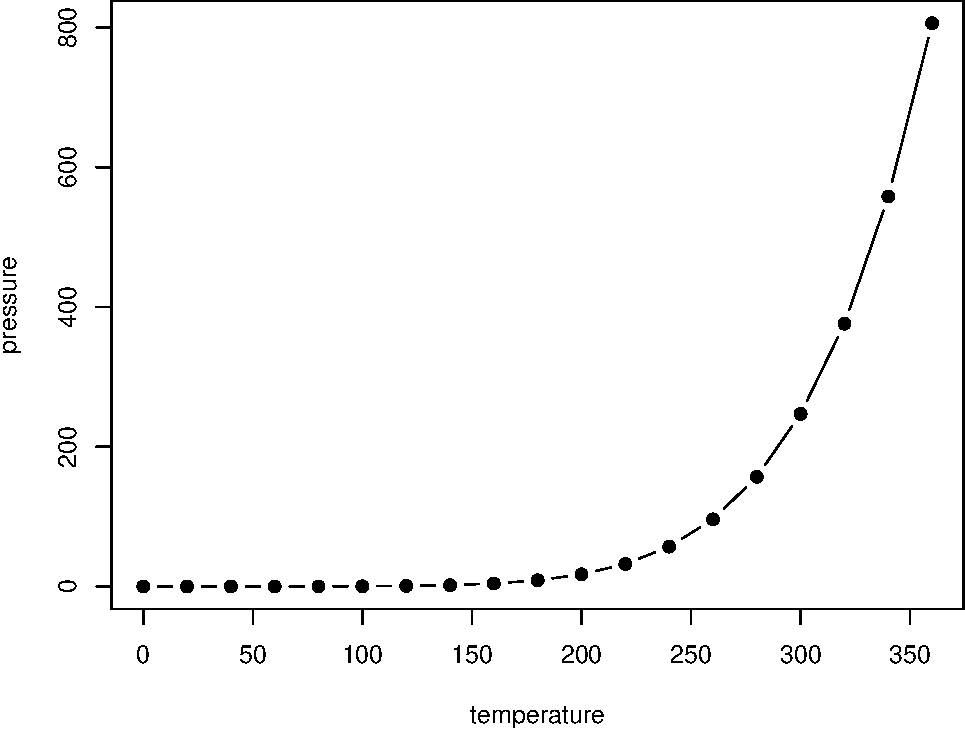
\includegraphics[width=0.8\linewidth]{bookdown-demo_files/figure-latex/nice-fig-1} 

}

\caption{Here is a nice figure!}\label{fig:nice-fig}
\end{figure}

Reference a figure by its code chunk label with the \texttt{fig:} prefix, e.g., see Figure \ref{fig:nice-fig}. Similarly, you can reference tables generated from \texttt{knitr::kable()}, e.g., see Table \ref{tab:nice-tab}.

\begin{table}

\caption{\label{tab:nice-tab}Here is a nice table!}
\centering
\begin{tabular}[t]{rrrrl}
\toprule
Sepal.Length & Sepal.Width & Petal.Length & Petal.Width & Species\\
\midrule
5.1 & 3.5 & 1.4 & 0.2 & setosa\\
4.9 & 3.0 & 1.4 & 0.2 & setosa\\
4.7 & 3.2 & 1.3 & 0.2 & setosa\\
4.6 & 3.1 & 1.5 & 0.2 & setosa\\
5.0 & 3.6 & 1.4 & 0.2 & setosa\\
\addlinespace
5.4 & 3.9 & 1.7 & 0.4 & setosa\\
4.6 & 3.4 & 1.4 & 0.3 & setosa\\
5.0 & 3.4 & 1.5 & 0.2 & setosa\\
4.4 & 2.9 & 1.4 & 0.2 & setosa\\
4.9 & 3.1 & 1.5 & 0.1 & setosa\\
\addlinespace
5.4 & 3.7 & 1.5 & 0.2 & setosa\\
4.8 & 3.4 & 1.6 & 0.2 & setosa\\
4.8 & 3.0 & 1.4 & 0.1 & setosa\\
4.3 & 3.0 & 1.1 & 0.1 & setosa\\
5.8 & 4.0 & 1.2 & 0.2 & setosa\\
\addlinespace
5.7 & 4.4 & 1.5 & 0.4 & setosa\\
5.4 & 3.9 & 1.3 & 0.4 & setosa\\
5.1 & 3.5 & 1.4 & 0.3 & setosa\\
5.7 & 3.8 & 1.7 & 0.3 & setosa\\
5.1 & 3.8 & 1.5 & 0.3 & setosa\\
\bottomrule
\end{tabular}
\end{table}

\hypertarget{citations}{%
\section{Citations}\label{citations}}

You can easily write citations using .bib files within this repository formatted using \href{http://www.bibtex.org/}{BibTEX}. For example, the \textbf{bookdown} package \citep{R-bookdown} in this reference book, which was built on top of R Markdown and \textbf{knitr} \citep{xie2015}.

\hypertarget{alt-text-for-accessibility}{%
\section{Alt Text for Accessibility}\label{alt-text-for-accessibility}}

\href{https://www.rstudio.com/blog/knitr-fig-alt/}{Use the knitr package to add alt text to graphics in R Markdown files}

\hypertarget{rendering-bookdown-to-build-publish}{%
\section{Rendering Bookdown to Build \& Publish}\label{rendering-bookdown-to-build-publish}}

In your Console, type either of these commands depending on which type of render you prefer:

\texttt{bookdown::render\_book("index.Rmd",\ "bookdown::gitbook")}
\texttt{bookdown::render\_book("index.Rmd",\ "bookdown::pdf\_book")}

To compile to PDF, you need XeLaTeX. It is recommended to install TinyTeX (which includes XeLaTeX): \url{https://yihui.name/tinytex/}.

\hypertarget{r}{%
\chapter{R and RStudio Installation}\label{r}}

\hypertarget{install-or-update-r}{%
\section{Install or Update R}\label{install-or-update-r}}

\textbf{R} is a programming language and environment used for statistical computing and grahics. For more information, please visit \href{https://www.r-project.org/about.html}{What is R}.

To install R, visit \href{https://cloud.r-project.org/}{cloud.r-project.org} to download the most recent version for your operating system.

\hypertarget{install-or-update-r-studio}{%
\section{Install or Update R Studio}\label{install-or-update-r-studio}}

RStudio is a software (considered an Integrated Development Environment, or IDE) that provides R programmers with an easy-to-use interface for coding in R.

\textbf{Note:} RStudio will not work without R installed, and you won't particularly enjoy using R without having RStudio installed. Be sure to install both!

\begin{itemize}
\item
  \textbf{New install:} To install RStudio, visit \href{https://www.rstudio.com/products/rstudio/}{rstudio.com/products/rstudio/}. Download the free (``Open Source Edition'') Desktop version for your operating system.
\item
  \textbf{Update:} If you already have RStudio and need to update: Open RStudio, and under `Help' in the top menu, choose `Check for updates.' If you have the most recent release, it will return `No update available. You are running the most recent version of RStudio.' Otherwise, you should follow the instructions to install an updated version.
\end{itemize}

Open RStudio (logo you'll click on shown below). If you are prompted to install Command Line Tools, do it.

\begin{center}
\includegraphics[width=4.97in]{images/rstudio} \end{center}

  \bibliography{book.bib,packages.bib}

\end{document}
